\documentclass[12pt,a4paper]{article}
\usepackage[margin=1in]{geometry}
\usepackage{amsmath,amssymb}
\newcommand{\E}{\mathbb{E}}
\newcommand{\indep}{\perp\!\!\!\perp}
\usepackage[UTF8,fontset=fandol]{ctex}
\usepackage{booktabs}
\usepackage{graphicx}
\usepackage{tikz}
\usetikzlibrary{arrows.meta, positioning}
\usepackage{float}
\usepackage{cite}
\usepackage[colorlinks=true,linkcolor=blue,citecolor=blue,urlcolor=blue]{hyperref}
\hypersetup{pdfborder={0 0 0},breaklinks=true,linktoc=all}
\usepackage{tocloft}
\setlength{\cftbeforesecskip}{3pt}
\setlength{\cftbeforesubsecskip}{1.5pt}
\setlength{\cftaftertoctitleskip}{0.8em}
\renewcommand{\cftsecfont}{\small}
\renewcommand{\cftsubsecfont}{\small}
\setcounter{tocdepth}{2}

\renewcommand{\abstractname}{摘要}
\makeatletter
\renewenvironment{abstract}{%
  \centerline{\cfttoctitlefont\abstractname}\par\vspace{0.8em}%
  \list{}{%
    \setlength{\leftmargin}{0pt}%
    \setlength{\rightmargin}{0pt}}%
  \item\relax\fontsize{13pt}{15.6pt}\selectfont}
 {\endlist}
\makeatother

\title{身体活动对心血管疾病风险的因果效应：\\基于倾向得分方法的识别、诊断与机制分析}
\author{盖烈森 \texttt{23307130013@m.fudan.edu.cn}}
\date{2026.6.5}

\begin{document}

\begin{titlepage}
\centering
\vspace*{2.8cm}
\begingroup
\linespread{1.25}\selectfont
{\LARGE\bfseries
身体活动对心血管疾病风险的因果效应\\[0.6em]
基于倾向得分方法的识别、诊断与机制分析
\par}
\endgroup
\vspace{2.8cm}
{\Large 盖烈森\par}
\vspace{0.8cm}
{\large \texttt{23307130013@m.fudan.edu.cn}\par}
\vspace{2.2cm}
{\Large 2026.6.5\par}
\vfill
\end{titlepage}

\newpage
\begin{abstract}
\noindent 本文在潜在结果框架下，利用 Ulianova 心血管公开数据集，研究身体活动对心血管疾病（CVD）风险的因果效应。在 DAG 与 backdoor 准则指导下明确 adjustment set，综合运用逆概率加权、g-formula、双重稳健估计及倾向得分匹配/分层等多种方法进行 triangulation，并系统开展倾向得分重叠、协变量平衡、BMI 中介分解与未测混淆敏感性等诊断与分析。结果表明，在控制主要混杂因素后，身体活动与 CVD 风险呈一致的保护性关联，多种识别—估计策略结论方向相同；保护效应主要体现为不经 BMI 中介的直接路径，BMI 所解释的机制份额有限。上述发现与国际流行病学文献关于体力活动可改变 CVD 危险因素的共识方向一致，支持在人群层面继续推广规律身体活动；但由于数据为横截面观察性设计，因果外推仍需谨慎，宜将结论理解为支持性而非确证性证据。

\vspace{0.6em}
\noindent\textbf{关键词：}身体活动；心血管疾病；因果推断；倾向得分；逆概率加权
\end{abstract}

\newpage
\tableofcontents

\newpage
\setcounter{page}{1}

\section{选题背景与研究问题}

\subsection{领域背景与已有证据}

全球范围内，体力活动不足与久坐行为持续上升，已被公认为可预防非传染性疾病——尤其是心血管疾病（CVD）——的重要危险因素 \cite{mi2025creview}。Mi 等人 \cite{mi2025creview} 在 \textit{Circulation Research} 的综述中指出，尽管过去数十年流行病学证据不断积累、各国公共卫生指南持续推广“每周至少 150 分钟中等强度有氧运动”等目标，美国及全球仍有大量人群未能达到推荐活动量，且少数族裔、女性与老年人等活动不足尤为突出。从机制上看，规律身体活动可通过改善内皮功能、降低 systemic inflammation、优化血压与血脂谱、提高心肺适能等途径保护心血管系统 \cite{mi2025creview}。因此，“增加活动能否降低 CVD 风险”既是公共卫生领域的核心命题，也是因果推断方法可以发挥作用的典型场景。

已有观察性研究为上述命题提供了大量支持性证据。Garcia 等人 \cite{garcia2023meta} 对 94 个前瞻性队列、逾三千万参与者进行剂量—反应 meta 分析，发现非职业性身体活动与全因死亡、CVD 死亡及多种癌症结局呈非线性负相关：从“不活动”到每周约 8.75 mMET-hours（相当于指南推荐的 150 分钟/周中等至高强度有氧运动）区间，风险降幅最大；在该剂量下，CVD 死亡的相对风险（RR）约为 0.71（95\% CI：0.66–0.77），全因死亡 RR 约为 0.69；若所有活动不足者均达到该水平，约 15.7\% 的过早死亡可被避免。Mi 等人 \cite{mi2025creview} 进一步归纳，观察性研究中更高活动量与更低死亡率及冠心病、缺血性卒中、心衰、房颤等多种 CVD 亚型风险之间的负向关联具有跨年龄、性别与基础健康状态的一致性；基于逾 200 万参与者、问卷评估活动的 pooled 分析显示，达到指南推荐活动量与约 22\% 的死亡率下降相关，而采用加速度计测量的研究往往报告更大的效应量。与此同时，机制层面的文献提示，活动对 CVD 的影响并非单一“总效应”所能概括：Chen 等人在中国成人中发现，活动经体脂肪百分比、血压与血脂等变量存在中介与修饰 \cite{chen2023pa}；Wang 等人报告，中—高强度休闲活动对高血压的效应部分经肥胖指标传递 \cite{wang2023obesity}；Hall 等人则指出，在考虑心肺适能（CRF）的中介作用后，与 cardiometabolic 健康相关的活动强度阈值可能发生变化 \cite{bjsports2023crf}。这些成果共同描绘了一幅“保护性关联 + 多通路机制”的图景，也为本文后续的中介分解提供了文献依据。

\subsection{观察性研究的局限与本文定位}

然而，从关联到因果，观察性 PA–CVD 研究仍面临若干结构性局限，这也是本文选题的出发点。活动水平并非随机分配：更年轻、代谢更健康、社会经济状况更好者往往更活跃，而这些因素同时影响 CVD 诊断，经典 confounding 使 crude 对比难以解释为因果效应 \cite{mi2025creview,hernan2024whatif}。在横截面或短随访设计中，反向因果同样棘手——已出现 CVD 症状或诊断者可能主动减少活动，从而夸大“活动者风险更低”的表象 \cite{mi2025creview}。当活动测量依赖自报问卷或粗分类时，回忆偏倚与误分类会进一步削弱效应估计的可信度；Mi 等人 \cite{mi2025creview} 指出，问卷与加速度计对同一活动量的效应估计可相差数倍，且不同设备、人群（如老年人）的测量可靠性亦存在差异。即便采用 Mendelian randomization（MR）等设计，因果结论也未必稳健：Qiu 等人 \cite{qiu2025mr} 基于欧洲 GWAS 的两样本 MR 发现，仅 vigorous physical activity（VPA）与 major coronary heart disease 存在 modest 的因果关联（IVW OR$=0.95$，95\% CI：0.91–0.99），而平均活动量及其他强度亚型与八种慢性病之间未见 substantial 因果联系——提示遗传工具对“一般性活动”的表征有限，MR 结论不能简单等同于“活动对 CVD 无因果效应”，但确实说明不同研究设计给出的因果证据强度并不一致。此外，Mi 等人 \cite{mi2025creview} 亦强调，直接证明 PA 降低 mortality 与 CVD 的 RCT 证据仍相对有限，长期依从性与伦理约束使大规模随机试验难以实施。综上，领域已有成果确立了 PA 的保护性方向与剂量线索，但在单一观察性数据集上如何于显式因果假设下估计可解释的 ACE、如何诊断识别条件、如何分解机制并评估残余混淆，仍有方法整合与透明报告的空间。

本文在上述背景下，利用 Ulianova 心血管公开数据集 \cite{ulianova2019kaggle} 开展一次完整的观察性因果分析流程。与既有文献相比，本文并不声称提供新的生物学发现或外推至全人群的因果定论，而侧重于在显式因果假设下完成一次方法学上透明、可复现的估计与诊断链条：在 DAG 与 backdoor 准则指导下明确 estimand 为 $\mathrm{ACE}=\E[Y(1)-Y(0)]$（风险差），并区分总效应 adjustment 与中介分解对 BMI 的不同处理 \cite{hernan2024whatif,vanderweele2015explanation}；在同一数据集上 triangulate IPW、g-formula、双重稳健 AIPW、线性模型及倾向得分匹配/分层等多种识别—估计策略 \cite{hernan2024whatif,rosenbaum1983central,robins1994estimation,shahu2023comparison}；系统报告 positivity 与协变量平衡诊断 \cite{chen2024iptw}；并在 VanderWeele 框架下分解 BMI 中介路径，结合 adjustment 规格敏感性、效应修饰与 E-value 讨论结论强度 \cite{vanderweele2015explanation,vanderweele2017evalue}。第 2 节阐述识别假设与估计原理；第 3 节给出多方法 ACE；第 4–5 节检验 positivity 与平衡——只有估计收敛且诊断通过，后续机制与敏感性讨论才有意义。

\subsection{数据、estimand 与因果结构}

数据来自 Kaggle 公开的 Ulianova 心血管体检数据集 \cite{ulianova2019kaggle}（原始文件 \texttt{cardio\_train.csv} 含 70{,}000 条记录）。分析前按血压（$ap\_hi\in[80,200]$、$ap\_lo\in[40,120]$ 且 $ap\_hi>ap\_lo$）、BMI（15–60）与身高（140–220 cm）剔除明显异常观测 1{,}608 条，清洗后保留 $N=68{,}392$ 条有效样本。需说明：同目录下另有 UCI Heart Disease 等小样本文件，并非本文所用数据。结局 $Y$ 为是否诊断 CVD（患病率 49.4\%）；处理 $A$ 为二值自报身体活动（活跃者占 80.3\%）。协变量涵盖年龄、性别、吸烟、饮酒、胆固醇、血糖与 BMI 等，与倾向得分/IPW 方法所需的多维 $L$ 结构相匹配，且变量均来自同一体检流程，定义一致。需要强调的是，该数据为横截面、活动为粗分类自报变量，无法区分活动强度、持续时间或客观测量，亦无法排除反向因果；因此本文结论应理解为“在该数据集与 stated 假设下的因果估计练习”，而非对 Garcia \cite{garcia2023meta} 等大型前瞻性 meta 结论的简单复现。

在潜在结果框架下，记 $A_i=1$ 表示个体 $i$ 保持身体活动，$Y_i=1$ 表示存在 CVD，$Y_i(a)$ 为处理 $a$ 下的潜在结局。目标 estimand 为平均因果效应
\[
\mathrm{ACE}=\E[Y_i(1)-Y_i(0)].
\]
若 $\mathrm{ACE}<0$，含义是：若将整个人群从不活跃（$A=0$）干预为活跃（$A=1$），平均 CVD 概率将下降 $|\mathrm{ACE}|$。这与“比较现有活跃/不活跃人群”的 associational 对比不同——后者混合了因果效应与选择性进入活动状态的偏倚 \cite{hernan2024whatif}。

图 \ref{fig:dag} 给出本文因果结构。年龄、性别、吸烟、饮酒、胆固醇与血糖既影响个体能否/是否保持活动，也直接影响 CVD 风险，形成 $A\leftarrow L\to Y$ 的 backdoor 路径；BMI 同样如此，并在生物学上可能部分充当 $A\to M\to Y$ 的中介 \cite{wang2023obesity,chen2023pa}。未测因素 $U$（如家族史、饮食模式、医疗可及性）若同时影响 $A$ 与 $Y$，则构成不可直接检验的残余混淆。主分析 adjustment set 为
\[
L=\{\text{年龄},\ \text{性别},\ \text{吸烟},\ \text{饮酒},\ \text{胆固醇},\ \text{血糖},\ \text{BMI}\},
\]
其选取依据是 backdoor 准则：在控制 $L$ 后，$A$ 与 $(Y(1),Y(0))$ 条件独立 \cite{hernan2024whatif,rosenbaum1983central}。主分析将 BMI 作为混淆控制以估计总效应；机制分析中再将 BMI 从 $L$ 中剥离，单独作为中介 $M$ 分解 NDE 与 NIE \cite{vanderweele2015explanation}。主分析 deliberately 不控制同期血压：在横截面数据里，血压既可能是活动长期作用的结果（中介），也可能反映已存在的心血管病理（混淆），纳入主模型会引入“过度控制中介”或“控制 collider”的风险 \cite{hernan2024whatif}；稳健性分析中再单独检验加入血压后的变化。

\begin{figure}[H]
\centering
\begin{tikzpicture}[
  >=Stealth, every node/.style={font=\small},
  var/.style={draw, rounded corners, minimum width=1.5cm, minimum height=0.65cm, align=center}
]
  \node[var] (U) at (0,2.3) {$U$};
  \node[var] (age) at (-3,1) {年龄};
  \node[var] (beh) at (-1,1) {吸烟/饮酒};
  \node[var] (meta) at (1.2,1) {胆固醇/血糖};
  \node[var] (A) at (-1,-0.2) {活动 $A$};
  \node[var] (M) at (1.5,-0.2) {BMI $M$};
  \node[var] (Y) at (0.3,-1.7) {CVD $Y$};
  \draw[->] (U) -- (A); \draw[->] (U) -- (Y);
  \draw[->] (age) -- (A); \draw[->] (age) -- (Y);
  \draw[->] (beh) -- (A); \draw[->] (beh) -- (Y);
  \draw[->] (meta) -- (A); \draw[->] (meta) -- (Y);
  \draw[->] (A) -- (Y); \draw[->] (A) -- (M); \draw[->] (M) -- (Y);
\end{tikzpicture}
\caption{因果图。$L$ 含年龄、性别、吸烟、饮酒、胆固醇、血糖及 BMI（总效应模型）；机制分析将 BMI 作为 $M$ 从 $L$ 中分离。}
\label{fig:dag}
\end{figure}

\section{识别假设与估计原理}

由观察数据识别 ACE，需要一组连接潜在结果与可观测变量的假设；只有在这些假设成立（或近似成立）时，后续的 IPW、g-formula 与倾向得分方法才具有因果解释 \cite{hernan2024whatif}。本节先阐述识别假设的含义与本文数据中的对应关系，再说明各估计量的构造原理及它们为何应当给出相近答案。

\subsection{识别假设}

一致性（consistency）要求：对每个个体，若其观测到的处理为 $A=a$，则观测结局 $Y$ 等于潜在结局 $Y(a)$，即 $Y=Y(A)=\sum_a Y(a)I(A=a)$ \cite{hernan2024whatif}。在本文中，$A$ 为二值自报活动状态，$Y$ 为 CVD 诊断；一致性隐含“活动”的定义在潜在结果与观测变量之间无歧义，且不存在同一 $A$ 值对应不同“处理版本”的情形。由于活动仅为粗分类自报变量，实际可能包含不同强度与类型，这一假设应理解为对“观测到的活跃/不活跃标签”的因果效应，而非对某一特定运动处方（如每周 150 分钟 MVPA）的效应 \cite{mi2025creview}。

稳定单元处理值假设（SUTVA）包含无干扰与处理版本唯一两部分 \cite{hernan2024whatif}。无干扰要求个体 $i$ 的潜在结局仅取决于其自身的 $A_i$，不受他人处理影响；在横截面体检数据中，个体间活动行为相互影响通常较弱，该假设相对合理。处理版本唯一则要求 $Y(1)$ 与 $Y(0)$ 明确定义——若“活跃”对不同个体意味着截然不同的活动模式，潜在结局的可解释性会下降。SUTVA 与一致性共同保证：我们估计的是 well-defined 的 $\E[Y(1)-Y(0)]$，而非混杂了测量误差与定义漂移的 associational 对比。

条件可交换性（conditional exchangeability，亦记为 ignorability 或“无未测混淆”）是观察性因果推断的核心：在控制 $L$ 后，潜在结局与处理独立，
\[
Y(1),Y(0)\indep A\mid L.
\]
其含义是：在 $L$ 取相同值的子人群中，活跃与否近似“可比较”，如同在该子群内做过条件随机化 \cite{hernan2024whatif,rosenbaum1983central}。图 \ref{fig:dag} 中，$L$ 阻断 $A\leftarrow L\to Y$ 等 backdoor 路径；若 additionally 存在 $U\to A$ 且 $U\to Y$ 而 $U$ 未被测量，则可交换性在真实数据生成机制下不成立，识别仅能在“$L$ 已充分”这一不可检验的前提下进行 \cite{hernan2024whatif}。本文将可测 $L$ 限于年龄、性别、吸烟、饮酒、胆固醇、血糖与 BMI，并承认家族史、饮食、社会经济地位等 $U$ 仍可能构成威胁——后文 E-value 分析即用于量化此类残余混淆需达到何种强度才能解释 away 估计 \cite{vanderweele2017evalue}。

positivity（overlap）要求：在 $L$ 的支撑上，
\[
0<\P(A=1\mid L=l)<1,
\]
即对每个协变量组合，活跃与不活跃个体均存在 \cite{hernan2024whatif,chen2024iptw}。若某些 $l$ 下 $\P(A=1\mid L=l)\approx 1$，则 $\E[Y(0)]$ 在该子群内缺乏经验支撑，IPW 中 $1/(1-e(L))$ 权重爆炸，匹配亦找不到对照。positivity 与可交换性不同：前者可通过倾向得分分布与协变量平衡图直接诊断（见第 4–5 节），后者无法由数据证明。本文样本中活跃者占 80.3\%，positivity 面临“处理组比例高、共同支撑区间偏窄”的现实，但不等于假设必然违背——关键在于 $\hat e(L)$ 在处理组与对照组间是否仍有重叠。

\subsection{估计原理}

在 consistency、SUTVA、$Y(a)\indep A\mid L$ 与 positivity 下，平均潜在结局可识别为
\[
\E[Y(a)]=\E\left[\E[Y\mid A=a,L]\right]=\E\left[\frac{I(A=a)\,Y}{\P(A=a\mid L)}\right],
\]
右式为 outcome regression（g-formula）与逆概率加权（IPW）两种策略 \cite{hernan2024whatif}。二者估计同一 $\E[Y(a)]$，但利用数据的方式不同：前者“先模型化 $Y$ 再对 $L$ 边际化”，后者“先模型化 $A$ 再重加权样本”。

逆概率加权（IPW）的直觉是构造一个伪总体，使其中 $A$ 与 $L$ 独立 \cite{chen2024iptw}。记 $e(L)=\P(A=1\mid L)$，则
\[
\E[Y(a)]=\E\left[\frac{I(A=a)\,Y}{\P(A=a\mid L)}\right]
\]
在有限样本中以 logistic 回归估计 $\hat e(L)=\widehat{\P}(A=1\mid L)$。对 $A_i=1$ 个体，稳定化权重常取 $w_i=\hat P(A=1)/\hat e(L_i)$；对 $A_i=0$，$w_i=(1-\hat P(A=1))/(1-\hat e(L_i))$，以减小权重方差 \cite{chen2024iptw}。ACE 估计为活跃组与对照组加权风险之差。IPW 仅要求倾向模型 $\hat e(L)$ 正确（或足够接近），不要求结局模型正确；但当 $e(L)$ 接近 0 或 1 时，权重极端，估计方差增大——这正是 positivity 诊断的重要性 \cite{chen2024iptw,hernan2024whatif}。

参数化 g-formula 直接对 $L$ 标准化 \cite{hernan2024whatif}：
\[
\E[Y(a)]=\sum_l \E[Y\mid A=a,L=l]\,\P(L=l),
\]
实践中以 logistic/线性模型拟合 $\widehat{\E}[Y\mid A,L]$，再对样本中 $L$ 的分布求平均。g-formula 不依赖倾向得分，但若 $\E[Y\mid A,L]$ 误设（例如忽略非线性或交互），仍会产生偏倚。当 IPW 与 g-formula 在 positivity 成立且模型均正确时收敛于同一 ACE；若二者明显分歧，往往提示倾向模型或结局模型至少一方严重误设 \cite{shahu2023comparison}。

双重稳健（augmented IPW, AIPW）估计将 outcome regression 与 IPW 结合 \cite{robins1994estimation,hernan2024whatif}。记 $\mu(a,L)=\E[Y\mid A=a,L]$，个体层估计为
\[
\hat\psi(a)=\hat\mu(a,L)+\frac{I(A=a)\bigl(Y-\hat\mu(a,L)\bigr)}{\hat e(L)},\qquad
\widehat{\mathrm{ACE}}=\overline{\hat\psi(1)}-\overline{\hat\psi(0)}.
\]
其“双重稳健”性体现在：若 $\hat e(L)$ 正确，则 IPW 残差项修正 $\hat\mu$ 的误差；若 $\hat\mu(a,L)$ 正确，则即使 $\hat e$ 有误，$\E[\hat\psi(a)]$ 仍等于 $\E[Y(a)]$ \cite{robins1994estimation,shahu2023comparison}。因此，当高维 $L$ 下单一线性/logistic 模型可能对 $e(L)$ 或 $\mu(a,L)$ 误设时，AIPW 提供额外保障——这也是本文同时报告 IPW、g-formula 与 AIPW 的理论动机。

倾向得分 $\pi(L)=\P(A=1\mid L)$ 将多维 $L$ 压缩为一维 \cite{rosenbaum1983central}。Rosenbaum 与 Rubin 证明：若 $Y(a)\indep A\mid L$，则 $Y(a)\indep A\mid \pi(L)$。匹配在 $\hat\pi(L)$ 相近的处理/对照间比较 $Y$；分层将样本按 $\hat\pi$ 分位数组，在组内估计效应再加权合并 \cite{rosenbaum1983central,chen2024iptw}。二者与 IPW 一样旨在阻断 backdoor 路径，但实现方式不同：匹配/分层更强调“局部可比”，IPW 更强调“全局重加权”。本文采用 1:1 最近邻匹配（caliper$=0.2\times$SD($\hat\pi$)）与五分位分层，以检验 ACE 是否依赖特定加权方案 \cite{rosenbaum1983central}。此外，线性概率模型（LPM）在控制 $L$ 后直接回归 $Y$ 于 $A$，在 $\mu(1,L)-\mu(0,L)$ 线性且可交换性成立时亦识别 ACE；其估计常与 g-formula 相近，但不具备 AIPW 的双重稳健性质 \cite{hernan2024whatif}。

综上，第 3 节将报告的 crude 风险差、IPW、g-formula、AIPW、LPM、PS 匹配与 PS 分层，在识别假设下目标均为 $\mathrm{ACE}=\E[Y(1)-Y(0)]$；若多种原理不同的估计收敛，则支持“偏倚方向一致且调整充分”的叙事，若分歧则提示模型或 positivity 问题 \cite{shahu2023comparison,hernan2024whatif}。

\section{总效应估计与结果解读}

第 2 节表明，在识别假设下 ACE 可由 IPW、g-formula、AIPW 及 PS 方法等多种途径估计；本节是全文的核心实证环节——首先报告 crude 与调整后 ACE，再检验七种方法是否收敛。若收敛，说明效应方向与量级对估计策略不敏感，第 4 节将进一步追问：这一收敛是否建立在 positivity 等可检验条件之上。

\subsection{Crude 对比与调整的必要性}

未调整前，不活跃组（$A=0$，$n=13{,}471$）CVD 率为 53.3\%，活跃组（$n=54{,}921$）为 48.5\%，粗风险差
\[
\mathrm{ACE}_{\text{crude}}=\bar Y_{A=1}-\bar Y_{A=0}=-0.0476\quad[{-0.0570},\ {-0.0382}],
\]
95\% 置信区间不含 0，associational 差异在统计上显著。活跃者 CVD 率更低，方向与 Garcia 等人 \cite{garcia2023meta} 及 Mi 等人 \cite{mi2025creview} 汇总的观察性保护性关联一致；但 crude 对比混合了两类不可交换因素：一是 $L$ 引起的 backdoor 偏倚，二是潜在的选择性进入活动状态。

加权前协变量差异（表 \ref{tab:balance} 左列）显示，活跃组在吸烟、饮酒上的 SMD 分别为 $+0.065$、$+0.064$，BMI 略低（SMD $=-0.035$），年龄略低（SMD $=-0.026$），胆固醇略高（SMD $=+0.022$）。吸烟/饮酒升高 CVD 风险，却更多集中在活跃组——若不控制 $L$，活跃组的 CVD 风险被人为抬高，crude 效应因此可能\textbf{低估}真实保护（绝对值偏大）。BMI 略低则相反，会部分抵消上述偏倚。净效应是 crude $|\mathrm{ACE}|$ 略大于调整后，与 backdoor 结构的定性预判一致，说明 crude 估计不能作为因果结论，必须进入 adjustment。

\begin{table}[H]
\centering
\caption{IPW 加权前后主要协变量 SMD（绝对值）}
\label{tab:balance}
\begin{tabular}{lcc}
\toprule
变量 & 加权前 $|\mathrm{SMD}|$ & 加权后 $|\mathrm{SMD}|$ \\
\midrule
吸烟     & 0.065 & $<0.001$ \\
饮酒     & 0.065 & $<0.001$ \\
BMI      & 0.035 & 0.003 \\
年龄     & 0.026 & $<0.001$ \\
胆固醇   & 0.022 & $<0.001$ \\
\bottomrule
\end{tabular}
\end{table}

\subsection{七种方法的 ACE 估计}

在控制 $L$ 后，表 \ref{tab:est} 与图 \ref{fig:forest} 汇总七种 ACE。按估计原理可分为三组：加权/回归类（IPW、AIPW、g-formula、LPM）给出 $-0.0439$ 至 $-0.0441$；PS 匹配 $-0.0435$（SE$=0.0030$，最窄）；PS 分层 $-0.0466$（SE$=0.0077$，最宽）。点估计落在 $[-0.047,\,-0.044]$ 的 3 个百分点区间内，全部 95\% CI 均不含 0——这是本文的首要实证发现：\textbf{对 $\hat e(L)$ 与 $\E[Y\mid A,L]$ 的不同利用方式并未导致结论分歧}，且保护效应在统计上稳健。

\begin{table}[H]
\centering
\caption{身体活动对 CVD 的 ACE 估计（$N=68{,}392$）}
\label{tab:est}
\begin{tabular}{lcc}
\toprule
方法 & ACE & 95\% CI \\
\midrule
粗风险差         & $-0.0476$ & [$-0.0570$, $-0.0382$] \\
IPW              & $-0.0440$ & [$-0.0527$, $-0.0354$] \\
双重稳健 AIPW    & $-0.0439$ & [$-0.0520$, $-0.0358$] \\
g-formula        & $-0.0439$ & [$-0.0530$, $-0.0349$] \\
LPM 回归         & $-0.0441$ & [$-0.0530$, $-0.0352$] \\
PS 匹配          & $-0.0435$ & [$-0.0494$, $-0.0376$] \\
PS 分层          & $-0.0466$ & [$-0.0616$, $-0.0315$] \\
\bottomrule
\end{tabular}
\end{table}

\begin{figure}[H]
\centering
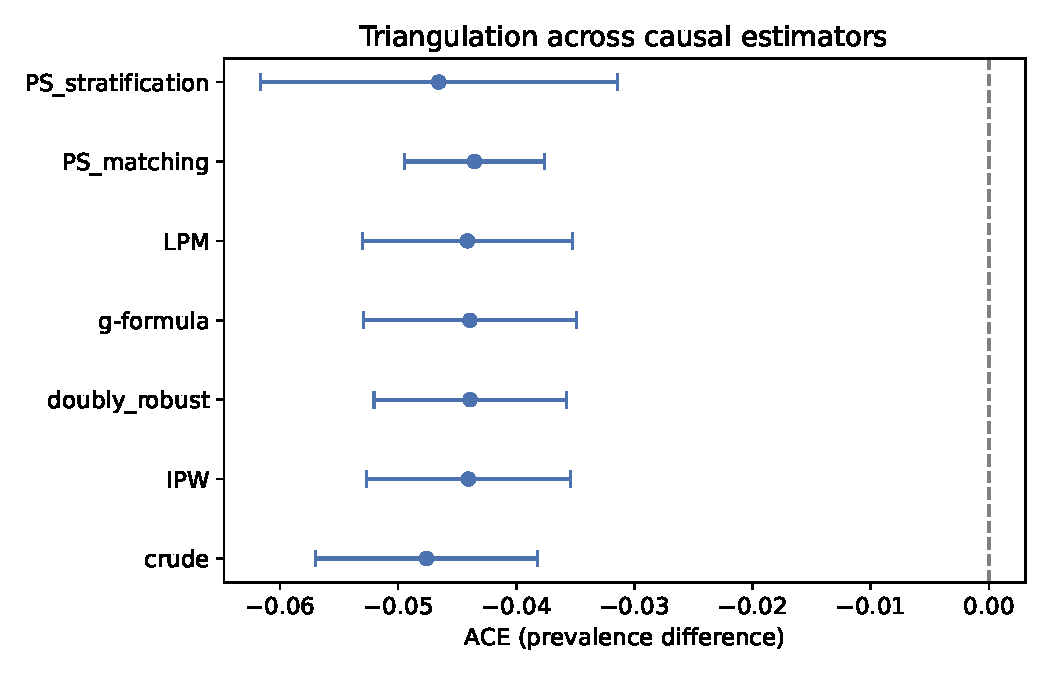
\includegraphics[width=0.88\textwidth]{../figures/forest_plot.pdf}
\caption{七种 ACE 估计的 forest plot（横轴为风险差，竖线为 95\% 置信区间）}
\label{fig:forest}
\end{figure}

以 IPW 点估计计，将不活跃组风险 $p_0=0.533$ 为参照，活跃组对应风险约 $p_0+\mathrm{ACE}\approx 0.489$，近似风险比 $\mathrm{RR}\approx 0.92$——保护方向与文献一致，但因结局为 CVD 患病率而非死亡、且活动仅为二值自报，效应量级不宜与 Garcia \cite{garcia2023meta} 的 CVD 死亡 RR（0.71）直接数值对比。就本数据集而言，将 80.3\% 的活跃者从不活跃反事实状态推至活跃，人群平均 CVD 概率约下降 4.4 个百分点，具有明确的公共卫生可解释性。

\subsection{多方法收敛的原理分析}

为何 IPW（依赖 $\hat e$）、g-formula（依赖 $\hat\mu$）、AIPW（二者结合）与 PS 匹配/分层（依赖 $\hat\pi$ 的局部可比）给出几乎相同的 ACE？从识别式看，它们目标均为 $\E[Y(1)]-\E[Y(0)]$。本数据中，IPW 与 g-formula 点估计仅差 0.0001（$-0.0440$ vs $-0.0439$），AIPW 与二者完全重合——这意味着倾向模型与结局模型在 ACE 层面\textbf{未出现足以撕裂结论的冲突}；若一方严重误设，IPW 与 g-formula 通常会明显分离 \cite{shahu2023comparison}。AIPW 未触发“单模型失效”的补偿机制，两套工作模型相互支持，这是 triangulation 的核心价值：不是重复同一回归，而是用不同识别路径交叉验证同一 estimand \cite{shahu2023comparison,hernan2024whatif}。

分方法看，IPW 与 g-formula 分别对应第 2.2 节两式——前者重加权样本使 $A\indep L$，后者对 $\E[Y\mid A,L]$ 边际化；二者在模型正确时等价，本结果正是这种等价性的经验体现。AIPW 在 Robins 意义下对 $\hat e$ 或 $\hat\mu$ 之一正确即一致 \cite{robins1994estimation}，与 IPW 重合说明至少未出现“两模型同时失效”的最坏情形。LPM 系数 $-0.0441$ 与 g-formula 几乎相同，符合线性 $\E[Y\mid A,L]$ 设定下二者等价的预期 \cite{hernan2024whatif}。

PS 匹配（$-0.0435$）略小于 IPW（$-0.0440$），标准误更窄（0.0030 vs 0.0044），与匹配在 $\hat\pi$ 相近者间做“局部随机化”、剔除 caliper 外不可比个体有关——匹配样本更同质，估计更精确，但可能略偏离全样本 ACE。PS 分层（$-0.0466$）点估计最接近 crude，区间最宽，因五分位层内 $A=0$ 个体稀少、层内方差大；这与第 4 节将讨论的“高活跃率下 positivity 区间偏窄”直接相关。尽管如此，分层估计仍落在其余方法 CI 内，说明效应并非某一加权方案的 artifact。

Crude 与调整后 ACE 的差异（$-0.0476$ vs $-0.0440$）亦可从 backdoor 结构理解：控制 $L$ 后，吸烟/饮酒对活跃组 CVD 风险的“向上拉拽”被剥离，ACE 绝对值略减小，符合 3.1 节对 confounding 方向的预判。综上，多方法 triangulation 支持：在控制 $L$ 且识别假设成立的前提下，活动使平均 CVD 风险下降约 4.4 个百分点。但收敛本身不能证明 positivity 或可交换性——第 4 节转向第 2.1 节中唯一可数据检验的 positivity。

\section{positivity 检验：倾向得分重叠}

第 3 节的 ACE 估计依赖 IPW 与 PS 方法，而二者均要求 positivity：在 $L$ 的支撑上 $0<e(L)<1$ \cite{hernan2024whatif,chen2024iptw}。若处理组与对照组的 $\hat e(L)$ 几乎不重叠，则 $\E[Y(0)]$ 在缺乏对照的 $\hat e$ 区域无法识别，第 3 节数值再一致也可能建立在“外推”而非“识别”之上。本节以倾向得分分布检验共同支撑是否成立。

\subsection{共同支撑与分布重叠}

记 $\hat e(L)=\widehat{\P}(A=1\mid L)$。图 \ref{fig:overlap} 展示 $A=0$ 与 $A=1$ 两组 $\hat e$ 的密度。由于样本中 80.3\% 为活跃者，logistic 倾向模型对多数个体给出较高的 $\hat e$：不活跃组（$n=13{,}471$）$\hat e$ 均值 0.802，范围 $[0.742,\,0.874]$；活跃组（$n=54{,}921$）均值 0.804，范围 $[0.745,\,0.879]$。共同支撑区为 $\hat e\in[0.745,\,0.874]$，99.99\% 个体落在此区间内。positivity 在经验上\textbf{未被违背}——对每个 $\hat e$ 水平，活跃与不活跃者均存在，IPW 权重不会因完全缺乏对照而系统性爆炸，PS 匹配亦能在 caliper 内找到对照。

\begin{figure}[H]
\centering
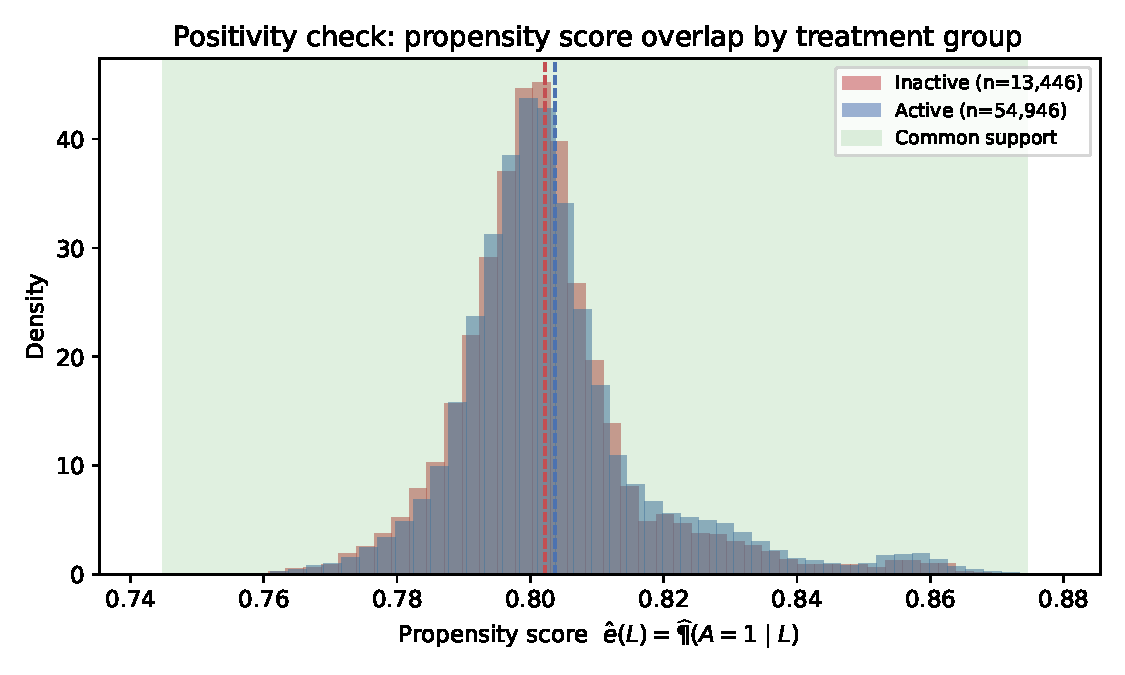
\includegraphics[width=0.92\textwidth]{../figures/ps_overlap.pdf}
\caption{positivity 检验：处理组与对照组倾向得分分布及共同支撑区（绿色）。虚线为各组 PS 均值。}
\label{fig:overlap}
\end{figure}

从权重结构可进一步理解上述结论。对不活跃个体，稳定化 IPW 权重为 $w_i=(1-\hat P(A=1))/(1-\hat e(L_i))$，其中 $\hat P(A=1)=0.803$。在 $\hat e$ 均值 0.802 处，$w_i\approx 0.197/0.198\approx 1.0$；对活跃个体，$w_i=\hat P(A=1)/\hat e(L_i)\approx 0.803/0.802\approx 1.0$。即使在共同支撑上界 $\hat e=0.874$，不活跃者权重约为 $0.197/0.126\approx 1.56$，仍属温和范围而非爆炸级。这说明第 3 节 IPW 估计并未被极端权重主导——positivity 不仅“形式上成立”，且在数值上对应可接受的权重分布 \cite{chen2024iptw}。

从原理看，positivity 检验回答的是“数据是否包含比较 $\E[Y(1)]$ 与 $\E[Y(0)]$ 所需的对照信息”，而非“可交换性是否成立”。重叠图至少排除了最致命的识别失败——完全无 overlap \cite{chen2024iptw}——从而为第 3 节 IPW/PS 估计提供必要（非充分）条件。

\subsection{高活跃率样本下的识别含义}

需要同时看到本数据的结构性特征：两组 $\hat e$ 均值几乎相同（0.802 vs 0.804），共同支撑区间宽度仅约 0.13——几乎所有人被预测为“高活动倾向”。这意味着，活动与否的变异主要来自 $L$ 内部的条件概率波动，而非 $\hat e$ 在 0 附近的广泛分散。ACE 的识别因此主要依赖“在相似 $\hat e$ 下、$L$ 仍驱动 $A$ 变化”的那部分外生变异；若 $L$ 对 $A$ 的解释力继续上升、$\hat e$ 进一步向 1 集中，positivity 将边际收紧 \cite{chen2024iptw}。

这一模式与高活跃率（80.3\%）样本一致：marginal 上“不活跃”者仅占 19.7\%，但 conditional 上仍可能存在 $e(L)<1$ 的个体——图 \ref{fig:overlap} 正是对此的检验。它直接解释了第 3 节中 PS 分层置信区间最宽（SE$=0.0077$）：五分位分层时，若干层内 $A=0$ 样本极少，层内风险差估计方差大；而全局 IPW 可利用全部 13{,}471 名不活跃者作为对照，标准误（0.0044）远小于 PS 分层。若 positivity 真正失败（例如 $\hat e\to 1$ 且无 $A=0$ 个体），我们将同时看到 overlap 消失、权重爆炸与 PS 匹配无法配对——本数据未出现这一模式。

positivity 与第 3 节结论的关系可概括为：第 3 节报告的多方法收敛，是在“共同支撑内 IPW/PS 识别可行”的前提下取得的；本节排除了“因缺乏对照而导致估计纯靠外推”的最严重情形。下一节将进一步检验：在共同支撑内，IPW 是否真正平衡了 $L$（表 \ref{tab:balance} 已预告加权后 $|\mathrm{SMD}|<0.003$），使第 3 节对 backdoor 路径的阻断在数据上可验证。

\section{协变量平衡与 IPW 的有效性}

第 4 节表明 positivity 在数据上成立，IPW/PS 估计具备识别的必要条件。但 positivity 只保证“对照存在”，并不保证 IPW 权重真正消除了 $L$ 在处理/对照间的分布差异——若加权后 $L$ 仍失衡，则 $Y(a)\indep A\mid L$ 所依赖的 backdoor 阻断在数据层面无法成立，第 3 节的 ACE 仍可能受残余 confounding 影响 \cite{rosenbaum1983central,chen2024iptw}。本节通过 love plot 与 SMD 量化 IPW 加权前后的协变量平衡，检验第 2.2 节 IPW 估计的“伪随机化”是否在可测 $L$ 上实现。

\subsection{IPW 加权的平衡原理}

Rosenbaum 与 Rubin \cite{rosenbaum1983central} 的核心结论是：若 $Y(a)\indep A\mid L$，则 $Y(a)\indep A\mid \pi(L)$，其中 $\pi(L)=\P(A=1\mid L)$。进一步地，在倾向得分相近的子群内，$L$ 的分布应在处理/对照间近似一致——这正是 IPW 有效性的可检验含义 \cite{chen2024iptw}。记稳定化权重 $w_i$ 如第 2.2 节，加权后第 $j$ 个协变量的标准化均值差（SMD）为
\[
\mathrm{SMD}_j=\frac{\bar L_{j,A=1}^{w}-\bar L_{j,A=0}^{w}}{s_j},
\]
其中 $\bar L^w$ 为加权均值，$s_j$ 为合并标准差。经验上 $|\mathrm{SMD}|<0.1$ 视为可接受平衡 \cite{chen2024iptw}；若加权后仍有 $|\mathrm{SMD}|>0.1$，则提示倾向模型遗漏重要协变量、positivity 仅在窄区间成立，或 IPW 权重不足以消除混杂 \cite{chen2024iptw,hernan2024whatif}。

需要强调：平衡诊断检验的是“可测 $L$ 上 backdoor 路径是否被阻断”，而非“可交换性是否成立”。$U$ 不可观测时，即使 $L$ 完全平衡，$Y(a)\indep A\mid L$ 仍可能被违背——第 7 节 E-value 将量化 $U$ 需多强才能解释 away 第 3 节估计 \cite{vanderweele2017evalue}。

\subsection{加权前后的协变量差异}

表 \ref{tab:balance_full} 与图 \ref{fig:love} 报告七个 adjustment 协变量的 SMD。加权前，活跃组与不活跃组在可测指标上存在系统性差异：吸烟（$|\mathrm{SMD}|=0.065$）与饮酒（0.065）差异最大，活跃组比例更高——与第 3.1 节对 confounding 方向的讨论一致；BMI（0.035）、年龄（0.026）、胆固醇（0.022）、血糖（0.020）亦有可见差异；性别（0.014）最小但仍非零。这些差异正是 crude 对比与调整后 ACE 不同的根源：若不加权，$A\leftarrow L\to Y$ 的 backdoor 路径未被阻断 \cite{hernan2024whatif}。

IPW 加权后，七个协变量的 $|\mathrm{SMD}|$ 均降至 0.003 以下（gender 0.001，smoke/alco $<0.001$，BMI 0.003，gluc 0.002，age/cholesterol $<0.001$）。从绝对量看，最大失衡从 0.065 压缩至不足 0.003，降幅超过 95\%。伪总体中 $A$ 与 $L$ 近似独立，说明 logistic 倾向模型 $\hat e(L)$ 在本数据上成功实现了“重加权后的协变量平衡”——这是 IPW 作为 backdoor adjustment 工具有效运作的直接证据 \cite{chen2024iptw}。

\begin{table}[H]
\centering
\caption{IPW 加权前后全部 adjustment 协变量 SMD}
\label{tab:balance_full}
\begin{tabular}{lrr}
\toprule
变量 & 加权前 SMD & 加权后 SMD \\
\midrule
吸烟（smoke）     & $+0.065$ & $-0.000$ \\
饮酒（alco）      & $+0.065$ & $-0.000$ \\
BMI              & $-0.035$ & $-0.003$ \\
年龄（age）       & $-0.026$ & $-0.000$ \\
胆固醇           & $+0.022$ & $+0.000$ \\
血糖（gluc）      & $-0.020$ & $-0.002$ \\
性别（gender）    & $+0.014$ & $+0.001$ \\
\bottomrule
\end{tabular}
\end{table}

\begin{figure}[H]
\centering
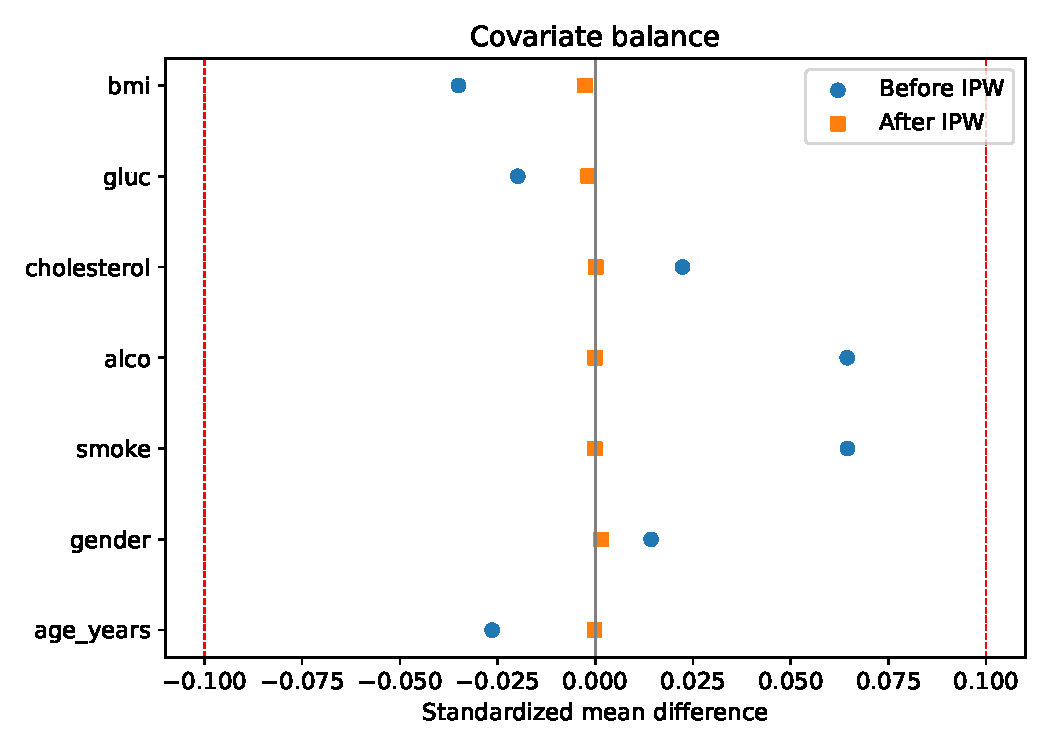
\includegraphics[width=0.88\textwidth]{../figures/love_plot.pdf}
\caption{IPW 加权前后协变量 SMD。红色虚线为 $\pm 0.1$ 阈值。}
\label{fig:love}
\end{figure}

\subsection{平衡诊断对第 3 节 ACE 的含义}

将第 4–5 节诊断与第 3 节结论对照，可形成一条完整的“可检验证据链”：第 4 节 positivity 图表明共同支撑成立（99.99\% 个体在 $\hat e\in[0.745,0.874]$ 内），IPW 权重无爆炸（上界处不活跃者权重 $\approx 1.56$）；本节 love plot 表明加权后 $L$ 平衡良好。二者共同支持：第 3 节 IPW ACE $=-0.0440$ 并非“缺乏对照”或“加权后仍严重失衡”下的伪估计 \cite{hernan2024whatif,chen2024iptw}。

当然，良好平衡不能证明 $U$ 不存在。吸烟/饮酒等“负向健康行为”在活跃组略多，IPW 已将其平衡——但若存在与活动、CVD 同时相关的未测 $U$（如家族史、饮食模式），可交换性仍可能被违背。positivity 与 balance 排除了可检验层面最严重的识别失败；第 6 节在总效应稳定的前提下追问机制，第 7 节进一步通过 adjustment 规格与 E-value 界定结论强度 \cite{vanderweele2017evalue}。

\section{机制分析：BMI 中介路径}

第 3–5 节确立：在控制 $L$ 后，活动对 CVD 的总效应 ACE $\approx -0.044$，且 IPW 识别条件在数据上可验证。下一问题是：这一保护效应有多少经 BMI 传递？Chen 与 Wang 等人在中国成人及休闲活动—高血压研究中均报告 PA 经肥胖相关指标存在中介 \cite{chen2023pa,wang2023obesity}；Hall 等人 \cite{bjsports2023crf} 则提示，考虑 CRF 后活动—健康关联的机制更为复杂。本节在 VanderWeele 回归式中介框架下 \cite{vanderweele2015explanation}，将 BMI 从 $L$ 中剥离为中介 $M$，分解自然直接效应（NDE）与自然间接效应（NIE），并与同期血压中介及敏感性分析对照。

\subsection{中介 estimand 与识别框架}

在图 \ref{fig:dag} 中，总效应模型将 BMI 纳入 $L$ 以阻断 $A\leftarrow M\to Y$ 的 backdoor；机制分析需改换 estimand：在控制 $L\setminus\{M\}=\{$年龄、性别、吸烟、饮酒、胆固醇、血糖$\}$ 后，定义
\[
\mathrm{NDE}=\E[Y(1,M(0))-Y(0,M(0))],\qquad
\mathrm{NIE}=\E[Y(0,M(1))-Y(0,M(0))],
\]
总效应 $\mathrm{TE}=\mathrm{NDE}+\mathrm{NIE}$ \cite{vanderweele2015explanation}。NDE 表示“阻断 $A\to M$ 路径时活动对 CVD 的效应”，NIE 表示“仅通过 BMI 变化传递的效应”。在线性 LPM 近似下，可分解为 $a$ 路径与 $b$ 路径：
\[
\mathrm{NIE}=a\times b,\quad
a=\E[M(1)-M(0)\mid L\setminus M],\quad
b=\E[Y(1,m)-Y(0,m)\mid L\setminus M,\,M=m].
\]
识别需额外假设：不存在 $M$ 与 $Y$ 之间的未测 confounder、$L\setminus M$ 已充分控制 $A$—$M$ 与 $A$—$Y$ 的 confounding，且 cross-world 独立性等 \cite{vanderweele2015explanation}。横截面下单次 BMI 测量亦无法捕捉动态体重变化——这些限制在解读 NIE 比例时需牢记。

\subsection{BMI 路径分解结果}

表 \ref{tab:med} 汇总分解结果（500 次 bootstrap CI）。$a$ 路径系数 $-0.183$：活跃者 BMI 平均低 0.18 单位（约 0.18 kg/m$^2$ 量级），活动确实与更低 BMI 相关。$b$ 路径 $+0.014$：在控制 $L\setminus M$ 后，BMI 每增 1 单位，CVD 风险差上升 1.4 个百分点。二者乘积 $\mathrm{NIE}=-0.183\times 0.014\approx -0.0026$ [$-0.0040$, $-0.0013$]：活动经 BMI 间接降低 CVD 风险约 0.26 个百分点。$\mathrm{NDE}=-0.0441$ [$-0.0530$, $-0.0362$]，占总效应 $\mathrm{TE}=-0.0468$ [$-0.0562$, $-0.0383$] 的约 94\%；间接路径约占 5.6\%。

\begin{table}[H]
\centering
\caption{BMI 中介路径分解（$L\setminus M$ 控制年龄、性别、吸烟、饮酒、胆固醇、血糖）}
\label{tab:med}
\begin{tabular}{lcc}
\toprule
效应 / 路径 & 估计 & 95\% CI \\
\midrule
$a$ 路径（$A\to M$）       & $-0.183$ & --- \\
$b$ 路径（$M\to Y\mid A$） & $+0.014$ & --- \\
NIE（间接效应）            & $-0.0026$ & [$-0.0040$, $-0.0013$] \\
NDE（直接效应）            & $-0.0441$ & [$-0.0530$, $-0.0362$] \\
总效应 TE                  & $-0.0468$ & [$-0.0562$, $-0.0383$] \\
间接效应占比               & 5.6\% & --- \\
\bottomrule
\end{tabular}
\end{table}

\begin{figure}[H]
\centering
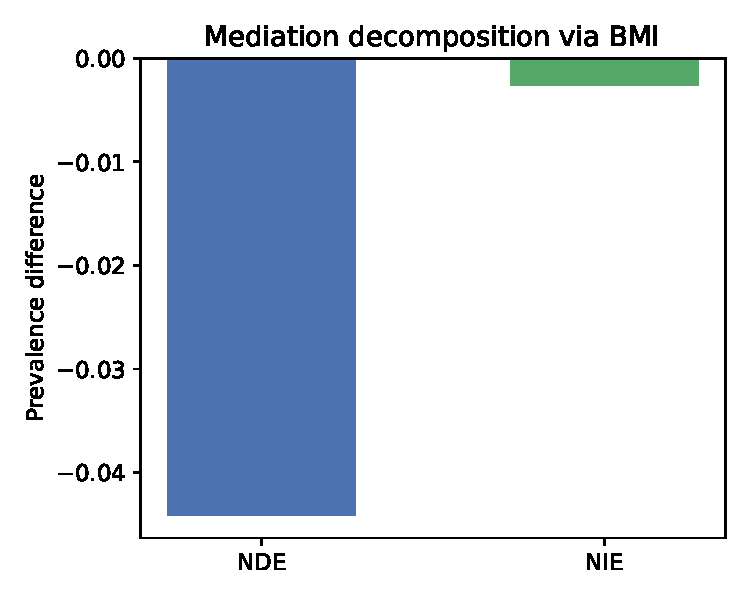
\includegraphics[width=0.48\textwidth]{../figures/mediation_decomp.pdf}
\hfill
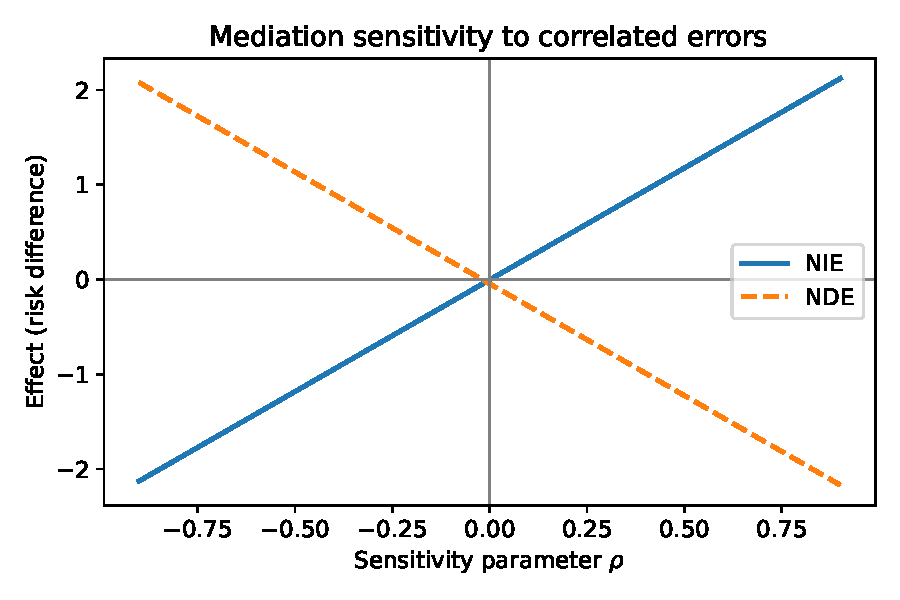
\includegraphics[width=0.48\textwidth]{../figures/mediation_sensitivity.pdf}
\caption{左：NDE 与 NIE 分解；右：中介敏感性——$\rho$ 为中介/结局模型残差相关系数时 NIE 的变化}
\label{fig:med}
\end{figure}

图 \ref{fig:med} 左直观展示 NDE 占主导。与第 3 节对照：剔除 BMI 的 IPW 总效应为 $-0.0468$（第 7 节），与中介分析 TE $=-0.0468$ 一致——因机制模型中 BMI 不再作为 confounder 控制，总效应略大于含 BMI 的主分析 ACE（$-0.0440$），符合“BMI 既是混淆也是中介”的 DAG 预期 \cite{vanderweele2015explanation}。NDE $=-0.0441$ 则与主分析 LPM/IPW 几乎相同，说明第 3 节报告的总效应本质上接近“不经 BMI 路径的直接效应”；BMI 通道仅贡献约 5.6\% 的额外保护。

\subsection{与文献及血压中介的对照}

NDE 占 94\% 是否与文献矛盾？并非如此。Chen 等人 \cite{chen2023pa} 在中国成人中报告 PA 经体脂肪、血压、血脂等多通路中介——本数据仅检验 BMI 单一路径，且为横截面二值活动，$a$ 路径虽显著但幅度有限。生物学上，活动还可通过改善内皮功能、降低 systemic inflammation、提高心肺适能等影响 CVD，这些机制不必然经 BMI 体现 \cite{bjsports2023crf,srep2025stiffness}。Wang 等人 \cite{wang2023obesity} 发现肥胖指标对 PA—高血压关联有中介，但本研究结局为 CVD 而非高血压，且 BMI 仅为肥胖的粗代理。

作为设计对照，若将中介换为同期收缩压 $ap\_hi$，$\mathrm{NIE}=+0.0006$，$\mathrm{NDE}=-0.0447$，总效应 $=-0.0441$——间接路径几乎为零。原因并非“血压不重要”，而是横截面血压同时反映长期活动效应与既有心血管病理（prevalent disease），单次体检无法识别“活动$\to$血压变化$\to$CVD”的动态链条 \cite{srep2025stiffness,hernan2024whatif}。这与纵向队列中报告显著血压中介的结果不矛盾，而是再次暴露横截面设计的局限。

\subsection{中介敏感性分析}

图 \ref{fig:med} 右报告 VanderWeele 式敏感性 \cite{vanderweele2015explanation}：若存在未测因素使中介模型与结局模型残差相关（参数 $\rho$），NIE 会随 $\rho$ 增大而上升。本数据中，中介/结局残差标准差分别为 5.02 与 0.47，当 $\rho\approx 0.001$ 时 NIE 可被完全抵消（$\rho_{\text{tip}}\approx 0.0011$）。由于 NIE 本身仅占 5.6\%，$\rho$ 需很小即可翻转间接效应——这主要威胁机制解释（“活动是否经 BMI 起作用”），而非总效应：扫描 $\rho$ 时 NDE 稳定在 $-0.044$ 左右，与第 3 节 IPW ACE 一致。因此，“活动降低 CVD”的结论不依赖 BMI 中介是否成立；即使 NIE 被未测因素完全解释，NDE 仍支持保护性总效应。

\section{异质性、adjustment 规格与未测混淆}

第 3 节给出总体 ACE，第 5–6 节表明识别诊断通过且 BMI 中介仅占一小部分。本节从三个角度进一步压力测试结论：效应是否在亚组间一致（异质性）？结论是否依赖 adjustment 规格（敏感性）？未测混淆需多强才能解释 away 估计（E-value）？三者共同界定第 3 节因果结论的外推边界 \cite{vanderweele2017evalue,hernan2024whatif}。

\subsection{年龄分层异质性}

按年龄四分位（Q1 最年轻 $\to$ Q4 最年长）重复 IPW，图 \ref{fig:age} 左报告各层 ACE。Q1 为 $-0.041$ [$-0.059$, $-0.023$]，Q2 为 $-0.039$ [$-0.057$, $-0.022$]，Q3 为 $-0.047$ [$-0.066$, $-0.029$]，Q4 为 $-0.050$ [$-0.068$, $-0.031$]。四层 95\% CI 均不含 0，且彼此高度重叠——保护效应在各年龄段均存在，未发现统计上显著的效应修饰。

从原理看，年龄分层 IPW 在每一层内重新估计 $\hat e(L)$ 并计算 ACE，相当于检验“保护效应是否仅由某一年龄组驱动”。Q4 点估计略大（$-0.050$ vs Q2 的 $-0.039$），或与高龄组 CVD 基线风险更高、活动带来的绝对风险下降空间更大有关 \cite{mi2025creview}；但层内样本量小于全样本、SE 约 0.009（全样本 IPW SE 为 0.004），置信区间较宽，不足以断言显著异质性。这一结果支持：第 3 节全样本 ACE 并非某一年龄段的 artifact，而是跨生命周期均存在的保护方向。

\subsection{吸烟的效应修饰}

在 LPM 中加入活动$\times$吸烟交互（控制与其余 $L\setminus\{\text{smoke}\}$），图 \ref{fig:age} 右报告分层效应。非吸烟者 ACE 为 $-0.0417$ [$-0.0510$, $-0.0324$]，吸烟者为 $-0.0734$ [$-0.1079$, $-0.0389$]；交互项系数 $-0.032$，$p=0.062$，边际显著。

如何理解？吸烟者基线 CVD 风险更高（$L$ 中 smoking 为强风险因素），活动带来的绝对风险下降空间更大，故子组 ACE 绝对值更大并不意外 \cite{medrxiv2023genePA}。但吸烟者 CI 很宽（上界 $-0.039$ 仍显著为负，下界 $-0.108$ 提示不确定性大），且 $p=0.062$ 未达常规 0.05 阈值——本文将其作为探索性发现，不据此断言“活动对吸烟者更有效”。重要的是：即使仅在非吸烟者中，ACE 仍为 $-0.042$ 且显著，第 3 节结论不依赖吸烟交互。

\begin{figure}[H]
\centering
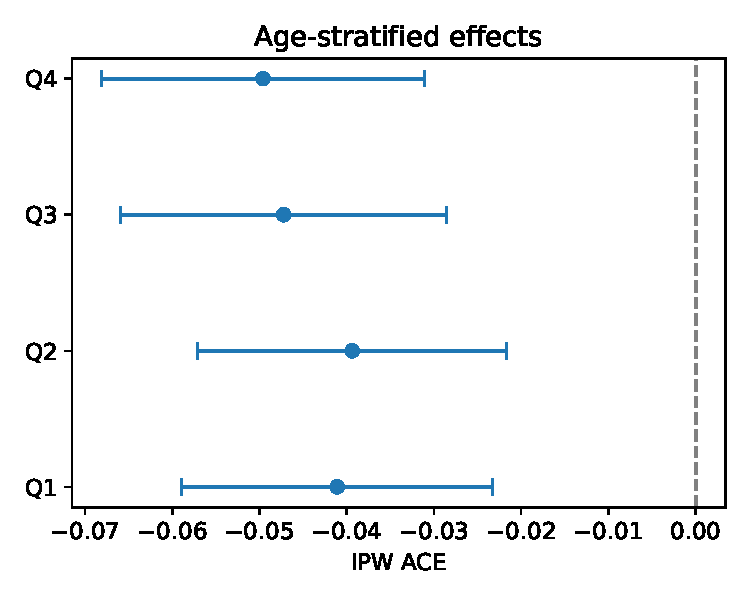
\includegraphics[width=0.46\textwidth]{../figures/age_heterogeneity.pdf}
\hfill
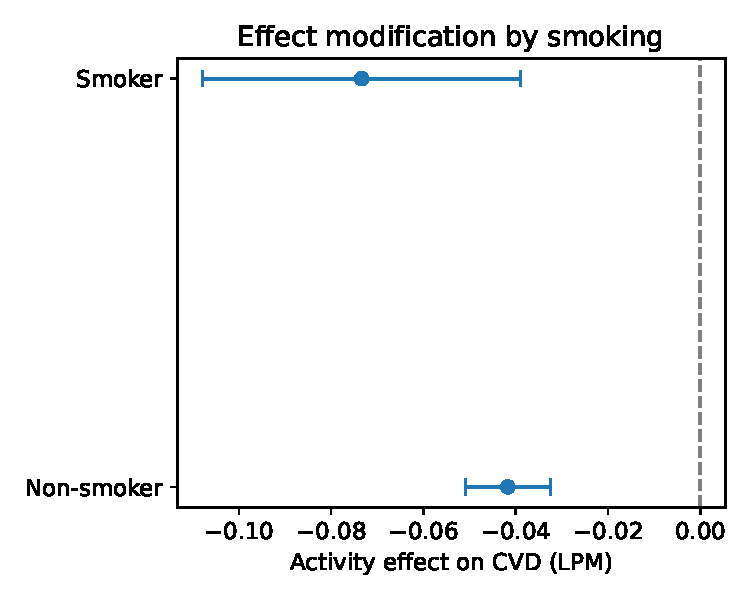
\includegraphics[width=0.46\textwidth]{../figures/effect_modification.pdf}
\caption{左：年龄四分位 IPW ACE 及 95\% CI；右：按吸烟分层的 LPM 效应及 95\% CI}
\label{fig:age}
\end{figure}

\subsection{adjustment set 规格敏感性}

adjustment set 的选择直接改变 estimand 含义 \cite{vanderweele2015explanation,hernan2024whatif}。图 \ref{fig:adj} 比较三种 IPW 规格（表 \ref{tab:adj}）：主分析（含 BMI）ACE $=-0.0440$ [$-0.0534$, $-0.0347$]；剔除 BMI 后为 $-0.0468$ [$-0.0557$, $-0.0379$]；额外加入收缩压/舒张压后为 $-0.0446$ [$-0.0530$, $-0.0361$]。

\begin{table}[H]
\centering
\caption{不同 adjustment set 下 IPW ACE}
\label{tab:adj}
\begin{tabular}{lcc}
\toprule
规格 & ACE & 95\% CI \\
\midrule
主分析（$L$ 含 BMI）       & $-0.0440$ & [$-0.0534$, $-0.0347$] \\
剔除 BMI                   & $-0.0468$ & [$-0.0557$, $-0.0379$] \\
额外加入血压（$ap\_hi$, $ap\_lo$） & $-0.0446$ & [$-0.0530$, $-0.0361$] \\
\bottomrule
\end{tabular}
\end{table}

\begin{figure}[H]
\centering
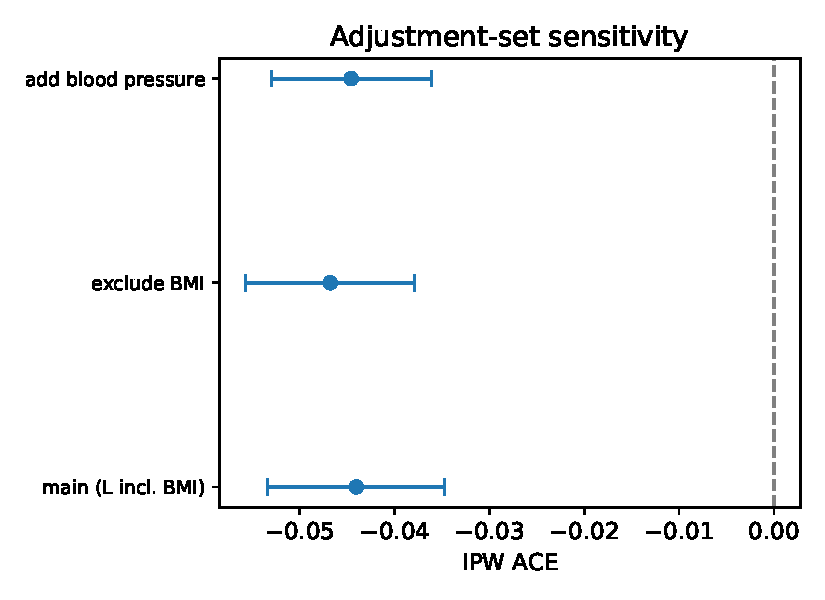
\includegraphics[width=0.65\textwidth]{../figures/adjustment_sensitivity.pdf}
\caption{不同 adjustment set 下 IPW ACE 及 95\% CI}
\label{fig:adj}
\end{figure}

剔除 BMI 后 ACE 绝对值增大约 0.003，与第 6 节机制分析一致：BMI 既是 $A\to Y$ 的 confounder 也是 $A\to M\to Y$ 的中介；主分析控制 BMI 估计的是“含 BMI 混淆路径的总效应”，剔除 BMI 则部分 opening 中介路径，TE 向 $-0.0468$ 偏移 \cite{vanderweele2015explanation}。加入血压后 ACE 几乎不变（$-0.0446$ vs $-0.0440$），说明同期血压未强烈驱动结论——既不支持“必须控制血压才有效”，亦不支持“控制血压后效应被大幅削弱”的极端情形，与第 1 节“主分析 deliberately 不控血压”的设计判断一致 \cite{hernan2024whatif}。三种规格 CI 高度重叠，第 3 节 ACE 对 reasonable adjustment 变动具有稳健性。

\subsection{E-value 与未测混淆}

可交换性 $Y(a)\indep A\mid L$ 不可检验，E-value 量化：需多强的未测混淆 $U$ 才能完全解释 away 观察效应 \cite{vanderweele2017evalue}。以 IPW 点估计 $\mathrm{ACE}=-0.0440$、不活跃组 CVD 率 $p_0=0.533$ 为基准，活跃组风险约 $p_1\approx 0.489$，近似 $\mathrm{RR}\approx 0.92$。E-value 点估计约为 1.40；针对 ACE 的 95\% 置信区间下界，E-value 约为 1.46——含义是：若存在未测 $U$，其与活动及 CVD 的关联强度（以 RR 尺度）均需达到约 1.4 量级，才可能完全抵消观察到的保护效应 \cite{vanderweele2017evalue}。

E-value 1.40 不算高：家族史、饮食模式、社会经济地位等 $U$ 与活动及 CVD 的关联完全可能达到这一量级 \cite{mi2025creview,hernan2024whatif}。因此，即便第 3–5 节多方法收敛、positivity 与平衡均通过，本文仍将因果结论定位为多方法、多诊断一致的 support 性证据，而非 RCT 级确证。E-value 与第 5 节“$U$ 仍可能威胁可交换性”的论述形成闭环：可检验条件良好，不可检验假设仍需谨慎。

将第 7 节与全文对照：第 3 节 ACE 稳定；第 4–5 节识别可检验条件成立；第 6 节机制以 NDE 为主；本节表明效应对年龄 robust、对 adjustment 规格不敏感，但 E-value 提示残余混淆不可忽视——这为第 8 节结论与局限提供了完整依据。

\section{结论与局限}

\subsection{主要结论}

本文在观察性数据中，围绕“身体活动是否因果性地降低 CVD 风险”开展了一次由识别假设、多方法估计、可检验诊断到机制与敏感性分析的完整因果推断流程。方法上，在 DAG 与 backdoor 准则指导下明确平均因果效应 estimand，依次采用逆概率加权、g-formula、双重稳健 AIPW、线性概率模型及倾向得分匹配/分层等多种原理不同的估计策略，并通过倾向得分重叠与协变量平衡检验 positivity 与加权有效性；在此基础上，进一步以 VanderWeele 框架分解 BMI 中介路径，结合 adjustment 规格变动、亚组分析与 E-value 评估结论强度 \cite{hernan2024whatif,vanderweele2015explanation,vanderweele2017evalue}。

主要发现可概括为三点。第一，在控制年龄、性别、吸烟、饮酒及主要代谢指标后，多种方法对总效应的估计方向与量级高度一致，均支持身体活动与 CVD 风险之间的 protective 关联——说明结论并非依赖某一特定加权或回归设定，而是在 stated 假设下具有较好的方法学稳健性 \cite{shahu2023comparison}。第二，positivity 与 IPW 后协变量平衡的诊断表明，识别所依赖的可检验条件在数据中得到满足，第 3 节的效应估计并非建立在“缺乏对照”或“加权后仍严重失衡”的脆弱基础之上 \cite{chen2024iptw,rosenbaum1983central}。第三，机制分析表明，保护效应以不经过 BMI 的直接路径为主，经 BMI 传递的间接效应占比较小；效应对不同年龄层均呈保护方向，对 adjustment 规格的 reasonable 变动亦不敏感，但 E-value 分析提示未测混淆仍可能削弱因果解释力度 \cite{vanderweele2017evalue}。

从现实意义看，本文结论与 Garcia 等人 \cite{garcia2023meta}、Mi 等人 \cite{mi2025creview} 等大量观察性证据所揭示的“体力活动不足是可改变的 CVD 危险因素”相一致：在人群层面推广规律身体活动、减少久坐，仍具有明确的公共卫生价值。本文的价值不仅在于给出一个 protective 的点估计，更在于示范如何在单一观察性数据集上，将因果 estimand 的界定、多方法 triangulation 与可检验诊断结合，使“关联”向“因果”的推断过程透明、可复现——这对今后同类体检数据或队列数据的分析具有参考意义。

\subsection{局限与展望}

本文仍存在若干局限，需在解读与推广时予以重视。数据为横截面设计，所有变量同一体检时点测量，无法排除“已患 CVD 者减少活动”的反向因果；活动为二值自报变量，未区分强度、频率与客观测量，与指南所指的 MVPA 剂量不能一一对应 \cite{mi2025creview}。可交换性假设本质上不可检验，尽管 positivity 与平衡诊断通过，家族史、饮食、社会经济地位等未测因素仍可能构成残余混淆，E-value 分析亦表明完全解释 away 观察效应所需的 confounding 强度并不极端 \cite{vanderweele2017evalue,hernan2024whatif}。中介分析依赖线性近似与横截面 BMI 测量，对“活动通过哪些生物学通路降低 CVD”的机制回答仍是初步的 \cite{vanderweele2015explanation}。

综上，本文将因果结论定位为多方法、多诊断一致的 support 性证据，而非随机试验级别的确证。未来研究可在纵向随访、自然实验或工具变量/MR 等设计下进一步验证；若结合加速度计等活动测量与更丰富的协变量，有望提高 estimand 的可解释性与外推强度。全部代码、数据、图表与数值输出已公开至 GitHub 仓库（见附录 \ref{app:repo}），便于复现与延伸。

\appendix

\section{图表一览}
\label{app:figures}

正文主要表格包括：表 \ref{tab:est}（七种 ACE 估计）、表 \ref{tab:balance} 与表 \ref{tab:balance_full}（协变量平衡）、表 \ref{tab:med}（BMI 中介分解）、表 \ref{tab:adj}（adjustment 敏感性）。主要插图如下。

\begin{table}[H]
\centering
\caption{正文插图索引}
\label{tab:figindex}
\begin{tabular}{clp{7.5cm}}
\toprule
图号 & 文件名 & 内容 \\
\midrule
\ref{fig:dag}   & （TikZ）       & 因果有向无环图 \\
\ref{fig:forest} & \texttt{forest\_plot.pdf} & 七种 ACE 估计 forest plot \\
\ref{fig:overlap} & \texttt{ps\_overlap.pdf} & 倾向得分重叠（positivity） \\
\ref{fig:love}   & \texttt{love\_plot.pdf} & IPW 加权前后 SMD \\
\ref{fig:med}    & \texttt{mediation\_*.pdf} & BMI 中介分解与 $\rho$ 敏感性 \\
\ref{fig:age}    & \texttt{age\_heterogeneity.pdf} 等 & 年龄分层与吸烟效应修饰 \\
\ref{fig:adj}    & \texttt{adjustment\_sensitivity.pdf} & adjustment set 敏感性 \\
\bottomrule
\end{tabular}
\end{table}

\section{代码仓库与复现说明}
\label{app:repo}

本项目的完整材料（数据集、分析脚本、数值输出、图表及 LaTeX 报告源文件）已上传至 GitHub 公开仓库：

\noindent\href{https://github.com/daomuyang/Liesen-Gai-Causal-Inference-Final-Project}{\nolinkurl{https://github.com/daomuyang/}\newline \nolinkurl{Liesen-Gai-Causal-Inference-Final-Project}}。

\subsection{仓库目录结构}

\begin{verbatim}
Liesen-Gai-Causal-Inference-Final-Project/
|-- data/
|   `-- cardio_train.csv      # Ulianova (70,000 raw rows)
|-- code/
|   `-- analysis.py           # main pipeline
|-- output/
|   |-- summary.json
|   |-- report_metrics.json
|   |-- estimates.csv
|   |-- balance.csv
|   `-- ...
|-- figures/                  # report figures (PDF)
|-- report/
|   `-- final_pj.tex
`-- FinalPJ_盖烈森.pdf        # compiled report
\end{verbatim}

\subsection{克隆与复现}

在本地克隆仓库并复现全部分析结果，可按以下步骤操作：
\begin{verbatim}
git clone \
  https://github.com/daomuyang/Liesen-Gai-Causal-Inference-Final-Project.git
cd Liesen-Gai-Causal-Inference-Final-Project

python3 -m venv .venv
source .venv/bin/activate        # Windows: .venv\Scripts\activate
pip install pandas numpy statsmodels scikit-learn matplotlib

MPLCONFIGDIR=.mplconfig python code/analysis.py
\end{verbatim}

运行成功后，\texttt{output/summary.json} 与 \texttt{figures/} 下的 PDF 将与正文一致；可在 \texttt{report/} 目录下执行 \texttt{xelatex final\_pj.tex}（两次）编译报告。分析样本量为原始 70{,}000 条经清洗后的 68{,}392 条；请勿将 \texttt{data/} 目录中其他 UCI Heart Disease 遗留文件误作本文数据源。

\begin{thebibliography}{99}

\bibitem{mi2025creview}
Mi MY, Perry AS, Krishnan V, Nayor M.
Epidemiology and cardiovascular benefits of physical activity and exercise.
\textit{Circulation Research}, 2025. doi: 10.1161/CIRCRESAHA.125.325526.

\bibitem{garcia2023meta}
Garcia L, et al.
Non-occupational physical activity and risk of cardiovascular disease, cancer and mortality outcomes: a dose--response meta-analysis of large prospective studies.
\textit{British Journal of Sports Medicine}, 57(15):979--989, 2023.

\bibitem{chen2023pa}
Chen X, et al.
The mediation and moderation effect among physical activity, body-fat percentage, blood pressure, and serum lipids among Chinese adults.
\textit{Nutrients}, 15(13), 2023.

\bibitem{wang2023obesity}
Wang Y, et al.
The mediation and interaction of the obesity index between moderate-vigorous recreational physical activity and hypertension.
\textit{Frontiers in Public Health}, 11:1288336, 2023.

\bibitem{bjsports2023crf}
Hall M, et al.
The physical activity intensity associated with cardiometabolic health when considering the mediating role of cardiorespiratory fitness.
\textit{British Journal of Sports Medicine}, 2023.

\bibitem{hernan2024whatif}
Hernán MA, Robins JM.
\textit{Causal Inference: What If}. Chapman \& Hall/CRC, 2024.

\bibitem{qiu2025mr}
Qiu P, Wu J, Li M, et al.
Causal inference between physical activity and chronic diseases: insights from a two-sample Mendelian randomization study.
\textit{Sports Medicine and Health Science}, 7(6):446--452, 2025.

\bibitem{ulianova2019kaggle}
Ulianova S.
Cardiovascular Disease Dataset. Kaggle, 2019.

\bibitem{shahu2023comparison}
Shahu A, et al.
Method comparison and estimation of causal effects of insomnia on health outcomes in a survey sampled population.
\textit{Scientific Reports}, 13:9831, 2023.

\bibitem{chen2024iptw}
Chesnaye NC, et al.
An introduction to inverse probability of treatment weighting in observational research.
\textit{Clinical Kidney Journal}, 2022.

\bibitem{vanderweele2015explanation}
VanderWeele TJ.
\textit{Explanation in Causal Inference: Methods for Mediation and Interaction}. Oxford University Press, 2015.

\bibitem{vanderweele2017evalue}
VanderWeele TJ, Ding P.
Sensitivity analysis in observational research: introducing the E-value.
\textit{Annals of Internal Medicine}, 167(4):268--274, 2017.

\bibitem{rosenbaum1983central}
Rosenbaum PR, Rubin DB.
The central role of the propensity score in observational studies for causal effects.
\textit{Biometrika}, 70(1):41--55, 1983.

\bibitem{robins1994estimation}
Robins JM, Rotnitzky A, Zhao LP.
Estimation of regression coefficients when some regressors are not always observed.
\textit{JASA}, 89(427):846--866, 1994.

\bibitem{srep2025stiffness}
Mediating role of arterial stiffness in the association between physical activity and cardiovascular disease risk.
\textit{Scientific Reports}, 2025.

\bibitem{medrxiv2023genePA}
Physical activity reduces the effect of adiposity genetic liability on hypertension risk in the UK Biobank cohort.
\textit{medRxiv}, 2023.

\end{thebibliography}

\end{document}
